

\section{OllyDbg}
Al abrir OllyDbg escogemos un archivo ya ensamblado para debuggear. Una vez
cargado el programa, si queremos un breakpoint podemos hacerlo desde la barra de
tareas o con F12. Al ejecutar el programa con breakpoints se detendrá al
conseguirse con el primer breakpoint, y para continuar la ejecución podemos
darle a continuar.

\begin{figure}[ht]
  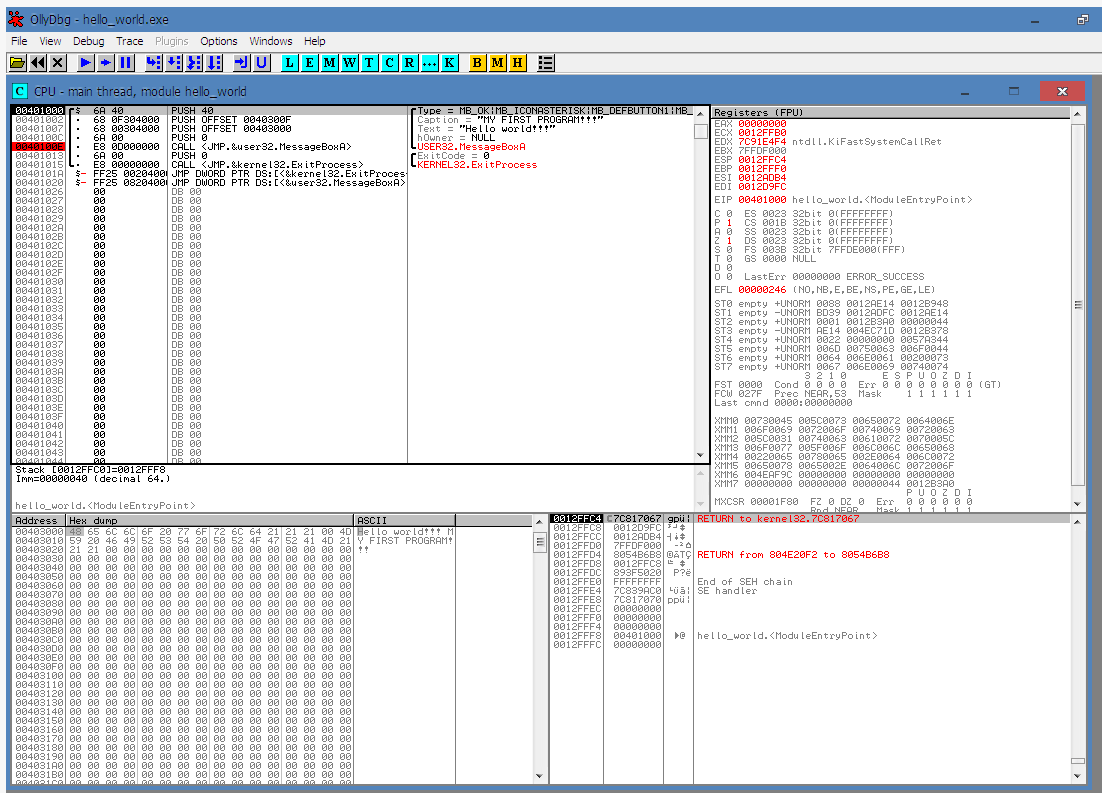
\includegraphics[width=\linewidth]{figs/fig6.png}
  \caption{Colocando breakpoint en OllyDbg}
  \label{fig:6}
\end{figure}

\begin{figure}[ht]
  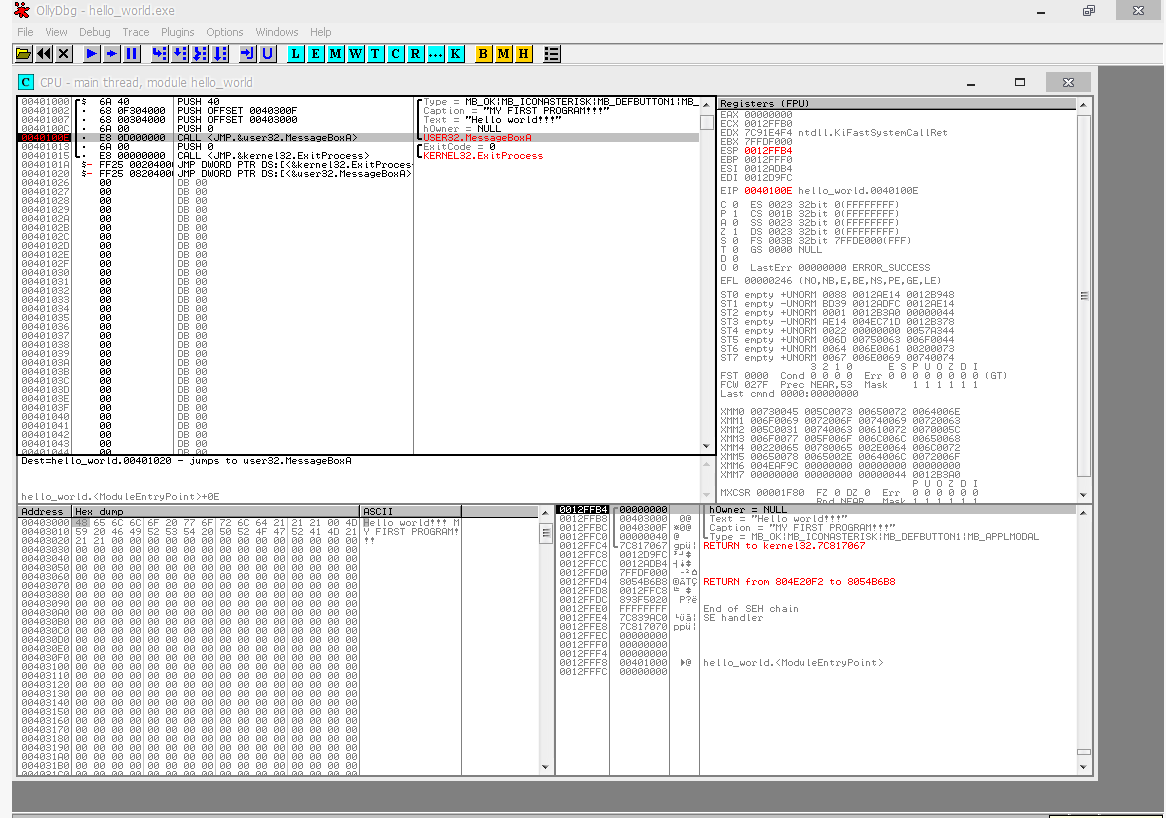
\includegraphics[width=\linewidth]{figs/fig7.png}
  \caption{Cayendo en breakpoint OllyDbg}
  \label{fig:7}
\end{figure}

\begin{figure}[ht]
  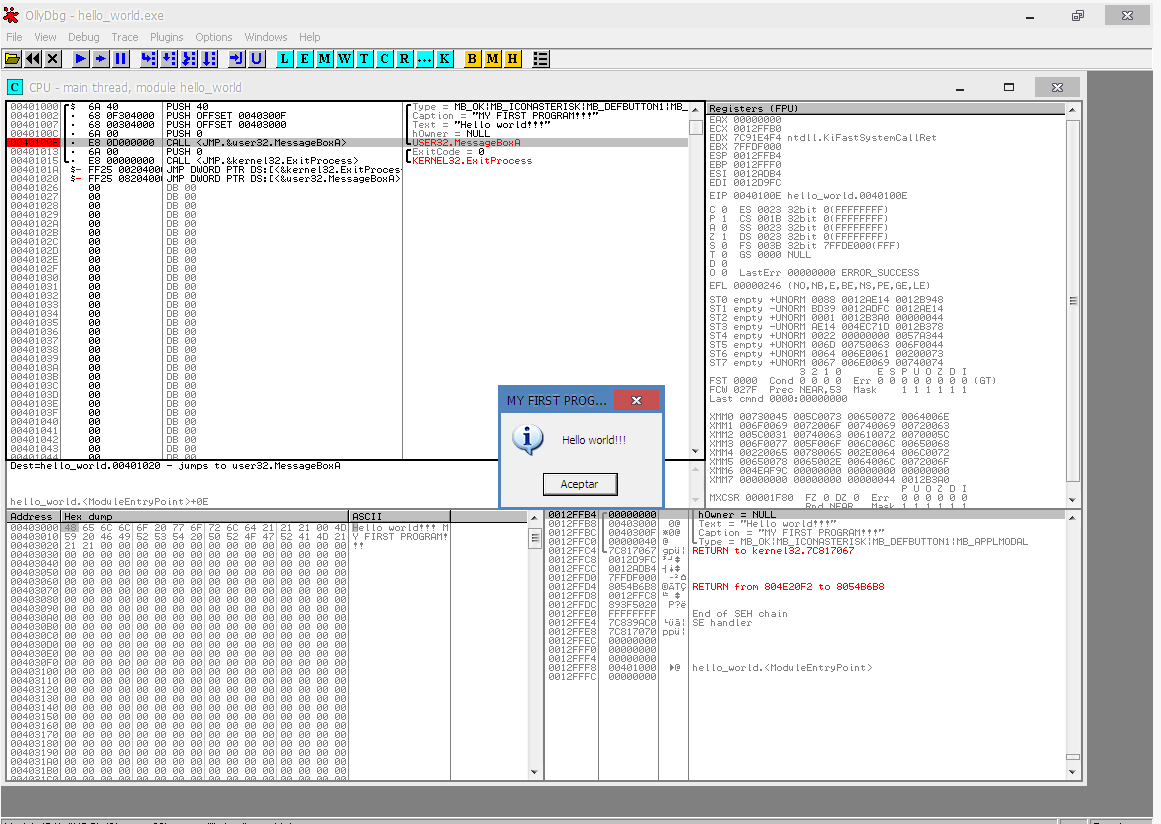
\includegraphics[width=\linewidth]{figs/fig8.png}
  \caption{Continuando ejecucion OllyDbg}
  \label{fig:8}
\end{figure}


